\section{Use Case Analysis}
Ziel: Abbildung der Realität in Anwendungsfalldiagramm. Dabei wird in der Regel ein konkretes Szenario beschrieben.
\begin{itemize}
	\item Use Case = Menge von Aktionssequenzen, die ein Nutzer oder externes System ausführt um ein bestimmtes Ziel zu erreichen. Beschreibt inhaltlich was beim Versuch der Zielerreichung passieren und schiefgehen kann.
	\item Helfen in der \textbf{Planungsphase}:\\
	- verdeutlichen wichtige Ziele des Produkts
	\item in der \textbf{Entwicklungsphase}\\
	- fassen Kernpunkte eines Features für Entwickler gut zusammen
	\item Erfassen der funktionalen R aus Sicht des Nutzers
\end{itemize}

\textbf{Actor:}
\begin{itemize}
	\item interagiert mit dem System; entweder Person oder wieder ein System
	\item gibt Input und erhält Output vom System
	\item extern; keine Kontrolle über den Use Case
	\item Vererbung möglich
	\item \textbf{Primär} und \textbf{Sekundär} Actor\\
	- Primär: will ein Ziel mithilfe des Systems erreichen\\
	- Sekundär: wird vom System benötigt um das Ziel des Primären zu erreichen
\end{itemize}

\begin{figure}[!h]
	\centering
	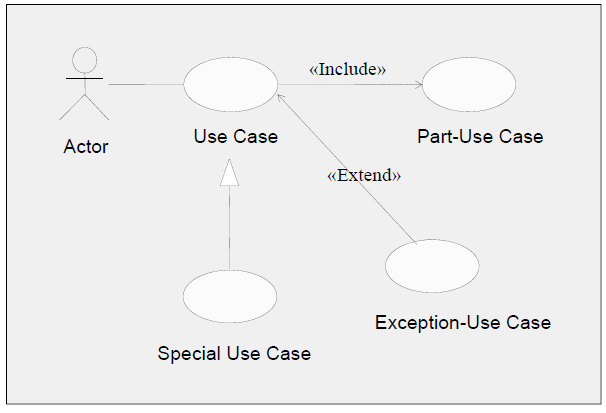
\includegraphics[scale=0.6]{img/elements_of_use_case.png}
	\caption{Elements of Use Case}
\end{figure}

Use Case begleitet die ganze Entwicklung. Wird \textit{realisiert} vom Design Model, \textit{Implementiert} vom Implementation Model und \textit{Verifiziert} vom Test Model.\\
\\
\textbf{Flow of Events}
\begin{itemize}
	\item \textbf{Happy Path} normal basic Flow
	\item alternative flows\\
	- exception flows for error situations\\
	- reguläre Alternativen ein Ziel zu erreichen\\
	- odd cases
\end{itemize}
\textbf{Scenario} = Sequenz von Aktionen die die Interaktion zwischen Actor und System beschreibt (quasi ein Element des Use Case)\\
\\
\textbf{Use Case Reports}\\
Beschreibt den Use Case im Detail. Einige Bestandteile nach Cockburn
\begin{itemize}
	\item Ziel
	\item Context of Use:  In welchem technischen Kontext tritt der Use Case auf?
	\item Level: Level of Detailt, Summary, Primary Task etc
	\item Folgende sind optional
	\item Actor
	\item Stakeholder
	\item Conditions
	\item Trigger
\end{itemize}
\textbf{Report ist wichtiger} als Use Case Model (<= Das Diagramm).
\\
Quasi Semi-Structured textuelle Beschreibung
\begin{itemize}
	\item Use Case Name
	\item Primary Actor
	\item Stakeholder and Interests
	\item Preconditions
	\item Success Garantie
	\item Trigger
	\item Main Success Scenario
	\items Extensions (zum main scenario)
\end{itemize}


Dazu gehören noch zusätzliche Spezi (mit Usability, Zuverlässigkeit Performance etc pp, quasi NFR zum Use Case) und Glossar -> Begriffsklärung. 

\newpage
\textbf{Use Case Analysis}
\begin{figure}[!h]
	\centering
	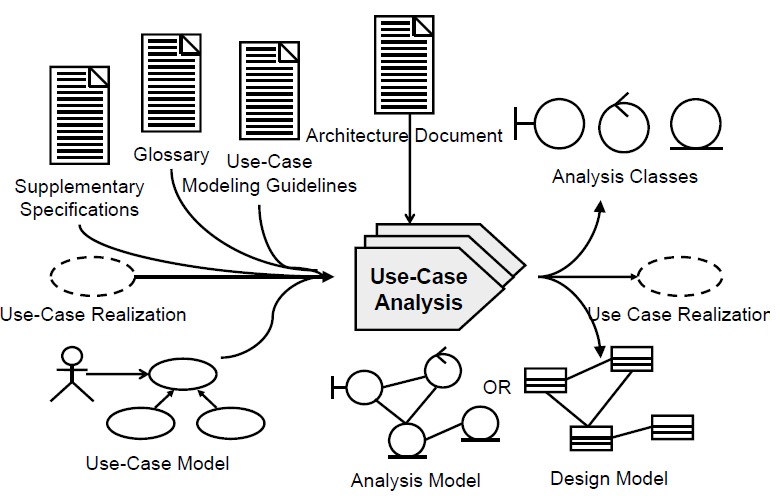
\includegraphics[scale=0.4]{img/use_case_analysis.png}
	\caption{Use Case Analysis}
\end{figure}

\textbf{Summary}\\
\begin{table}[!h]
	\begin{tabular}{p{20em}|p{20em}}
		Vorteile & Nachteile\\
		\hline
		zeigen functional R in einfacher, verständlicher Art & zeigen ausschließlich functional R\\
		Erstellen Framework\footnote{Ich denke hiermit ist eher ein 'Rahmen' gemeint.} für non-functional R und Projekt Details. & 
	\end{tabular}
\end{table}

\subsection{Glossar}
\begin{itemize}
	\item \textbf{Sequenzdiagramm} = Graphische Darstellung eines Szenarios, das Interaktion zw. Objekten zeitlich darstellt
	\begin{figure}[!h]
		\centering
		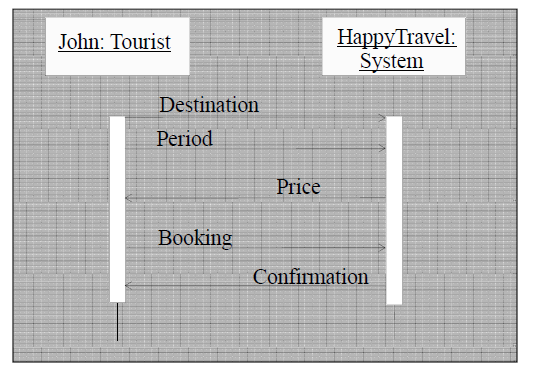
\includegraphics[scale=0.5]{img/ex_sequence_diagram.png}
		\caption{Ex Sequence Diagram}
	\end{figure}
	\item \textbf{Collaboration Diagram} = Interaktionsdiagramm - zeigt eine Sequenz von Nachrichten, die eine Operation oder Transaktion implementieren
	\begin{figure}[!h]
		\centering
		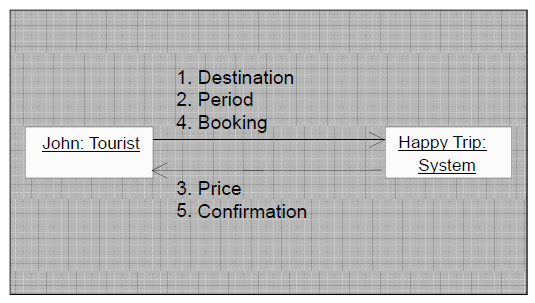
\includegraphics[scale=0.5]{img/ex_collaboration_diagram.png}
		\caption{Ex Collaboration Diagram}
	\end{figure}
\end{itemize}

